\documentclass{article}

% Language setting
% Replace `english' with e.g. `spanish' to change the document language
\usepackage[utf8]{inputenc}
\usepackage[spanish]{babel}

% Set page size and margins
% Replace `letterpaper' with `a4paper' for UK/EU standard size
\usepackage[letterpaper,top=2cm,bottom=2cm,left=3cm,right=3cm,marginparwidth=1.75cm]{geometry}

% Useful packages
\usepackage{amsmath}
\usepackage{graphicx}
\usepackage[colorlinks=true, allcolors=blue]{hyperref}
\usepackage{newunicodechar}
\newunicodechar{ε}{\ensuremath{\varepsilon}}

\title{Práctica 3 TALF}
\author{José Ruiz Pareja}

\begin{document}
\maketitle



\section{Autómata con pila no determinista:}
Construye un APND en JFLAP que reconozca el lenguaje L = {0^n 1^2^n : n > 0}


\begin{center}
    \centering
    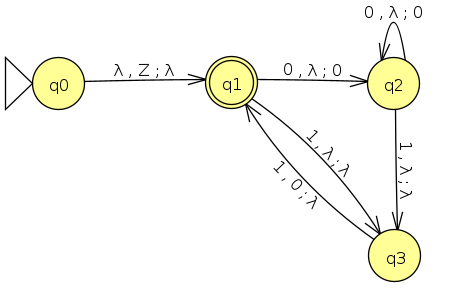
\includegraphics[width=0.5\linewidth]{APDN1.png}
\end{center}

Verifica el autómata construido con 6 cadenas de ejemplo.

Cadenas de ejemplo:
\begin{center}
    \centering
    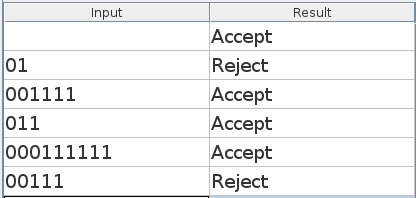
\includegraphics[width=0.5\linewidth]{EjemplosAPND.png}
\end{center}



Haz lo mismo en Python, definiendo el autómata en el JSON e instanciándolo con los mismos ejemplos.

APND definido en el JSON:
\begin{verbatim}
    {
    "name" : "APND1",
    "hint" : "",
    "e.g." : [],
    "representation" : {
      "K" : ["q0", "q1"],
      "I" : ["0", "1"],
      "S" : ["0", "1"],
      "s" : "q0",
      "F" : ["q0"],
      "t" : [[["q0", "0", "ε"],["q1", "0"]],
             [["q0",  "1", "ε"],["q2", "ε"]],
             [["q1",  "0", "ε"],["q1", "0"]],
             [["q1",  "1", "ε"],["q2", "ε"]],
             [["q2",  "1", "0"],["q0", "ε"]]]
      }
  }
\end{verbatim}

Y probamos con los mismos ejemplos:
\begin{center}
    \centering
    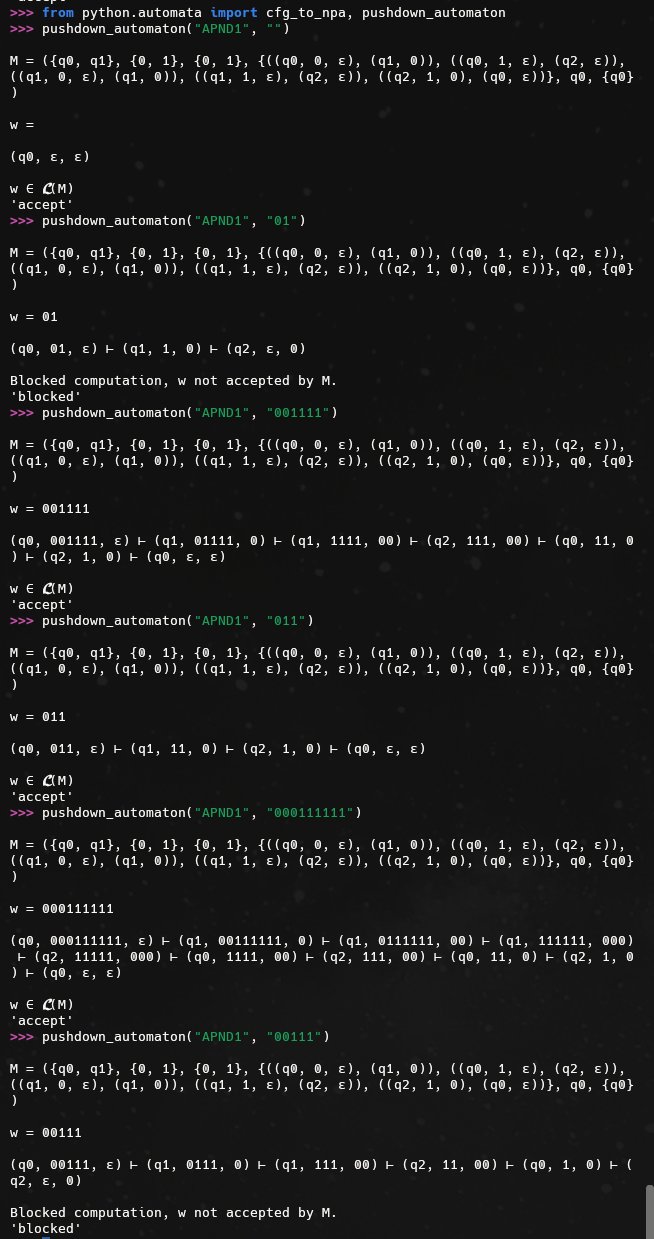
\includegraphics[width=0.5\linewidth]{ejemplosPythonAPND1.png}
\end{center}


\section{Máquina de Turing:}
Define en JFLAP la MT que define la suma de dos números naturales.

Si copiamos la MT de la solucion del ejercico 12 tal cual, quedaría tal que asi:
\begin{center}
    \centering
    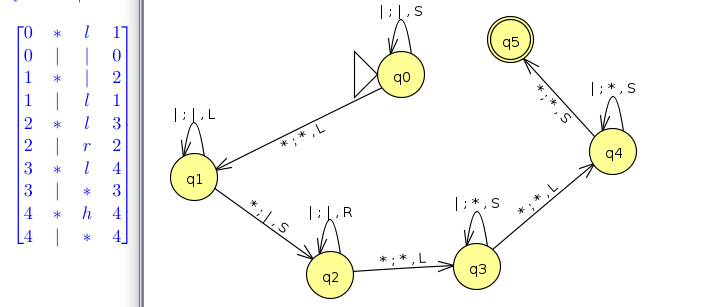
\includegraphics[width=0.5\linewidth]{MT1JFLAP.png}
\end{center}

Sin embargo, en JFLAP la máquina de Turing se posiciona al inicio delante de la cadena
\begin{center}
    \centering
    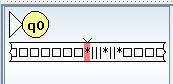
\includegraphics[width=0.5\linewidth]{posicionMT1.png}
\end{center}
Por lo que, para que la máquina funcione, se deberian de invertir todos los desplazamientos de la máquina (izquierda por derecha y viceversa). La MT en JFLAP tendría el siguiente aspecto con los desplazamientos ya invertidos:

\begin{center}
    \centering
    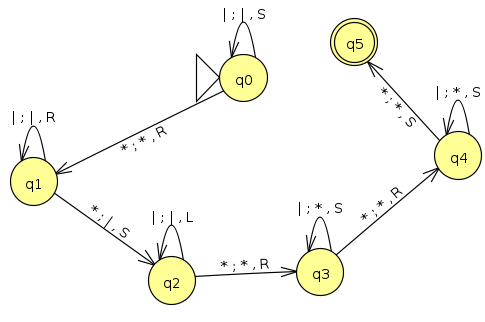
\includegraphics[width=0.5\linewidth]{MT2JFLAP.png}
\end{center}

De este modo, ya se puede realizar la funcion suma (2+1):
\begin{center}
    \centering
    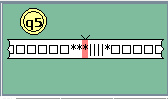
\includegraphics[width=0.5\linewidth]{sumaMT.png}
\end{center}

Comprueba su correcto funcionamiento comparándolo con su ejecución en Python.

En python, comprobamos que con la misma entrada $"*|||*||*"$, funciona y además no hace falta invertir los desplazamientos.

\begin{center}
    \centering
    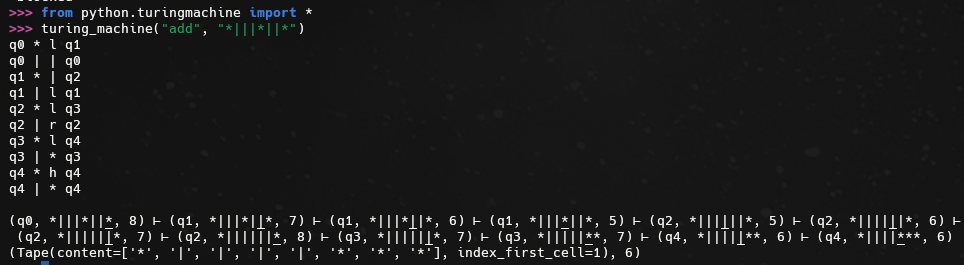
\includegraphics[width=0.5\linewidth]{pythonSumaMT.png}
\end{center}

\newpage

\section{Función recursiva}

Sabemos que $suma(n_1 + n_2) = n_1 + n_2$ es una funcion recursiva, ya que se puede definir como:
\\
$suma(n)= \{\pi_1^1 | sucesor_3\}(n)$
\\

Por lo que la suma de 3 numeros se podría definir como:
\\
$suma(suma(n_1 + n_2) + n_3) = suma(n_1 + n_2) + n_3 = n_1 + n_2 + n_3$ 
\\
La suma de 3, 2 y 1 quedaría como:
$suma(suma(1 + 2) + 3) = suma(1 + 2) + 3 = 3 + 3 = 6$ 


Compara tu evaluación con su ejecución en Python.
\begin{center}
    \centering
    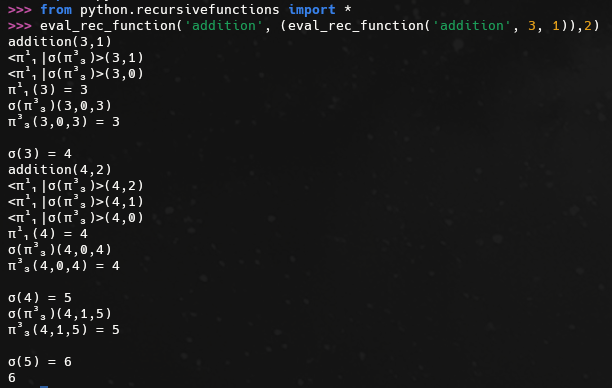
\includegraphics[width=0.75\linewidth]{pythonSumade3.png}
\end{center}

Como podemos ver, en python tambien se resuelve por partes la funcion recursiva.


\end{document}
